\chapter{Plataformas de desarrollo y herramientas utilizadas}
\label{cap:capitulo3}

Para hacer realidad todo lo mencionado en capítulos anteriores, se usaron diversos recursos ingenieriles que hicieron posible el proyecto. A continuación, se detallará cada uno de ellos.

\section{Lenguajes de programación}
\label{sec:lenguajes_programacion}

\subsection{Python}
\label{subsec:python}

A día de hoy, considerado el lenguaje de programación más popular \cite{tiobe}, se ideó en 1991 por Guido van Rossum y se desarrolló en la Python Software Foundation \cite{python-history}. Es interpretado, es decir, usa un programa que traduce las líneas de código para la máquina en tiempo de ejecución (lo cual lo hace más intuitivo pero menos eficiente). Además, permite la programación orientada a objetos en alto nivel, lo que ofrece gran dinamismo a la hora de usarlo \cite{python-def} \cite{compiled-vs-interpreted}.\\

Debido a su amplia popularidad, podemos acceder a una gran variedad de módulos y utilidades desarrollados por la comunidad, los cuales se integran perfectamente en la resolución de nuestro problema. Entraremos en más detalles en apartados posteriores.\\

\begin{code}[H]
\begin{lstlisting}[language=Python]
#! /usr/bin/env python

if __name__ == "__main__":
    print("Hello world!")
\end{lstlisting}
\caption[Hello world en Python]{\emph{Hello world} en Python}
\label{cod:helloworld_python}
\end{code}

\subsection{C++}
\label{subsec:cplusplus}

Seguido muy de cerca en fama, se encuentra el lenguaje de programación creado por Bjarne Stroustrup, en los laboratorios Bell en 1971. En este caso es compilado, lo que implica la traducción y enlazado previo a la ejecución. De corte más eficiente que Python, también permite la programación orientada a objetos. Se sitúa a medio camino entre un lenguaje de alto nivel y uno de bajo nivel \cite{c-history}.\\

\begin{code}[H]
\begin{lstlisting}[language=C++]
#include <iostream>

int main(int argc, char ** argv) {
    std::cout << "Hello World!" << std::endl;
    return 0;
}
\end{lstlisting}
\caption[Hello world en C++]{\emph{Hello world} en C++}
\label{cod:helloworld_cplusplus}
\end{code}

\section{\ac{ROS}}
\label{sec:ros}

Si se habla de robótica, se habla de \ac{ROS}, ya que es el medio predilecto para el desarrollo de soluciones de este ámbito, pero, ¿qué es exactamente \ac{ROS}?.\\

Se trata de un \emph{middleware}, es decir, una infraestructura software situada entre el sistema operativo y el desarrollador, que incluye una serie de módulos y funcionalidades enfocadas al desarrollo de aplicaciones robóticas \cite{middleware-def} \cite{ros-def}. La idea detrás, busca estandarizar soluciones que no dependan de los drivers de cada sensor y actuador presentes. De forma general, se trata de una arquitectura basada en nodos que se comunican entre sí, transmitiendo una serie de mensajes propios, a través de canales compartidos llamados \emph{topics}.\\

Entre las herramientas usadas en este proyecto, se encuentran las siguientes.

\begin{figure} [H]
	\begin{center}
	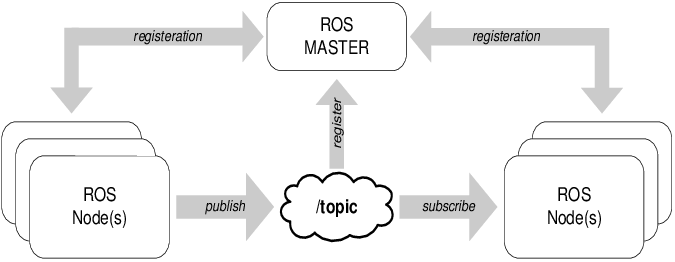
\includegraphics[height=3.25cm]{imagenes/cap3/1_ros_esquema.png}
	\end{center}
	\caption[Esquema ROS Noetic]{Esquema ROS Noetic}
	\label{fig:ros}
\end{figure}

\subsection{Gazebo 11}
\label{subsec:gazebo}

Se trata del simulador sobre el cual se desarrolla el proyecto. Concretamente consta de un conjunto de módulos optimizados para desarrollar aplicaciones robóticas, a través del previamente mencionado \ac{ROS} \cite{gazebo-def}.\\

Esta herramienta, nos permite visualizar en directo, el comportamiento del dron frente a los diversos escenarios que se planteen.

\begin{figure} [H]
	\begin{center}
	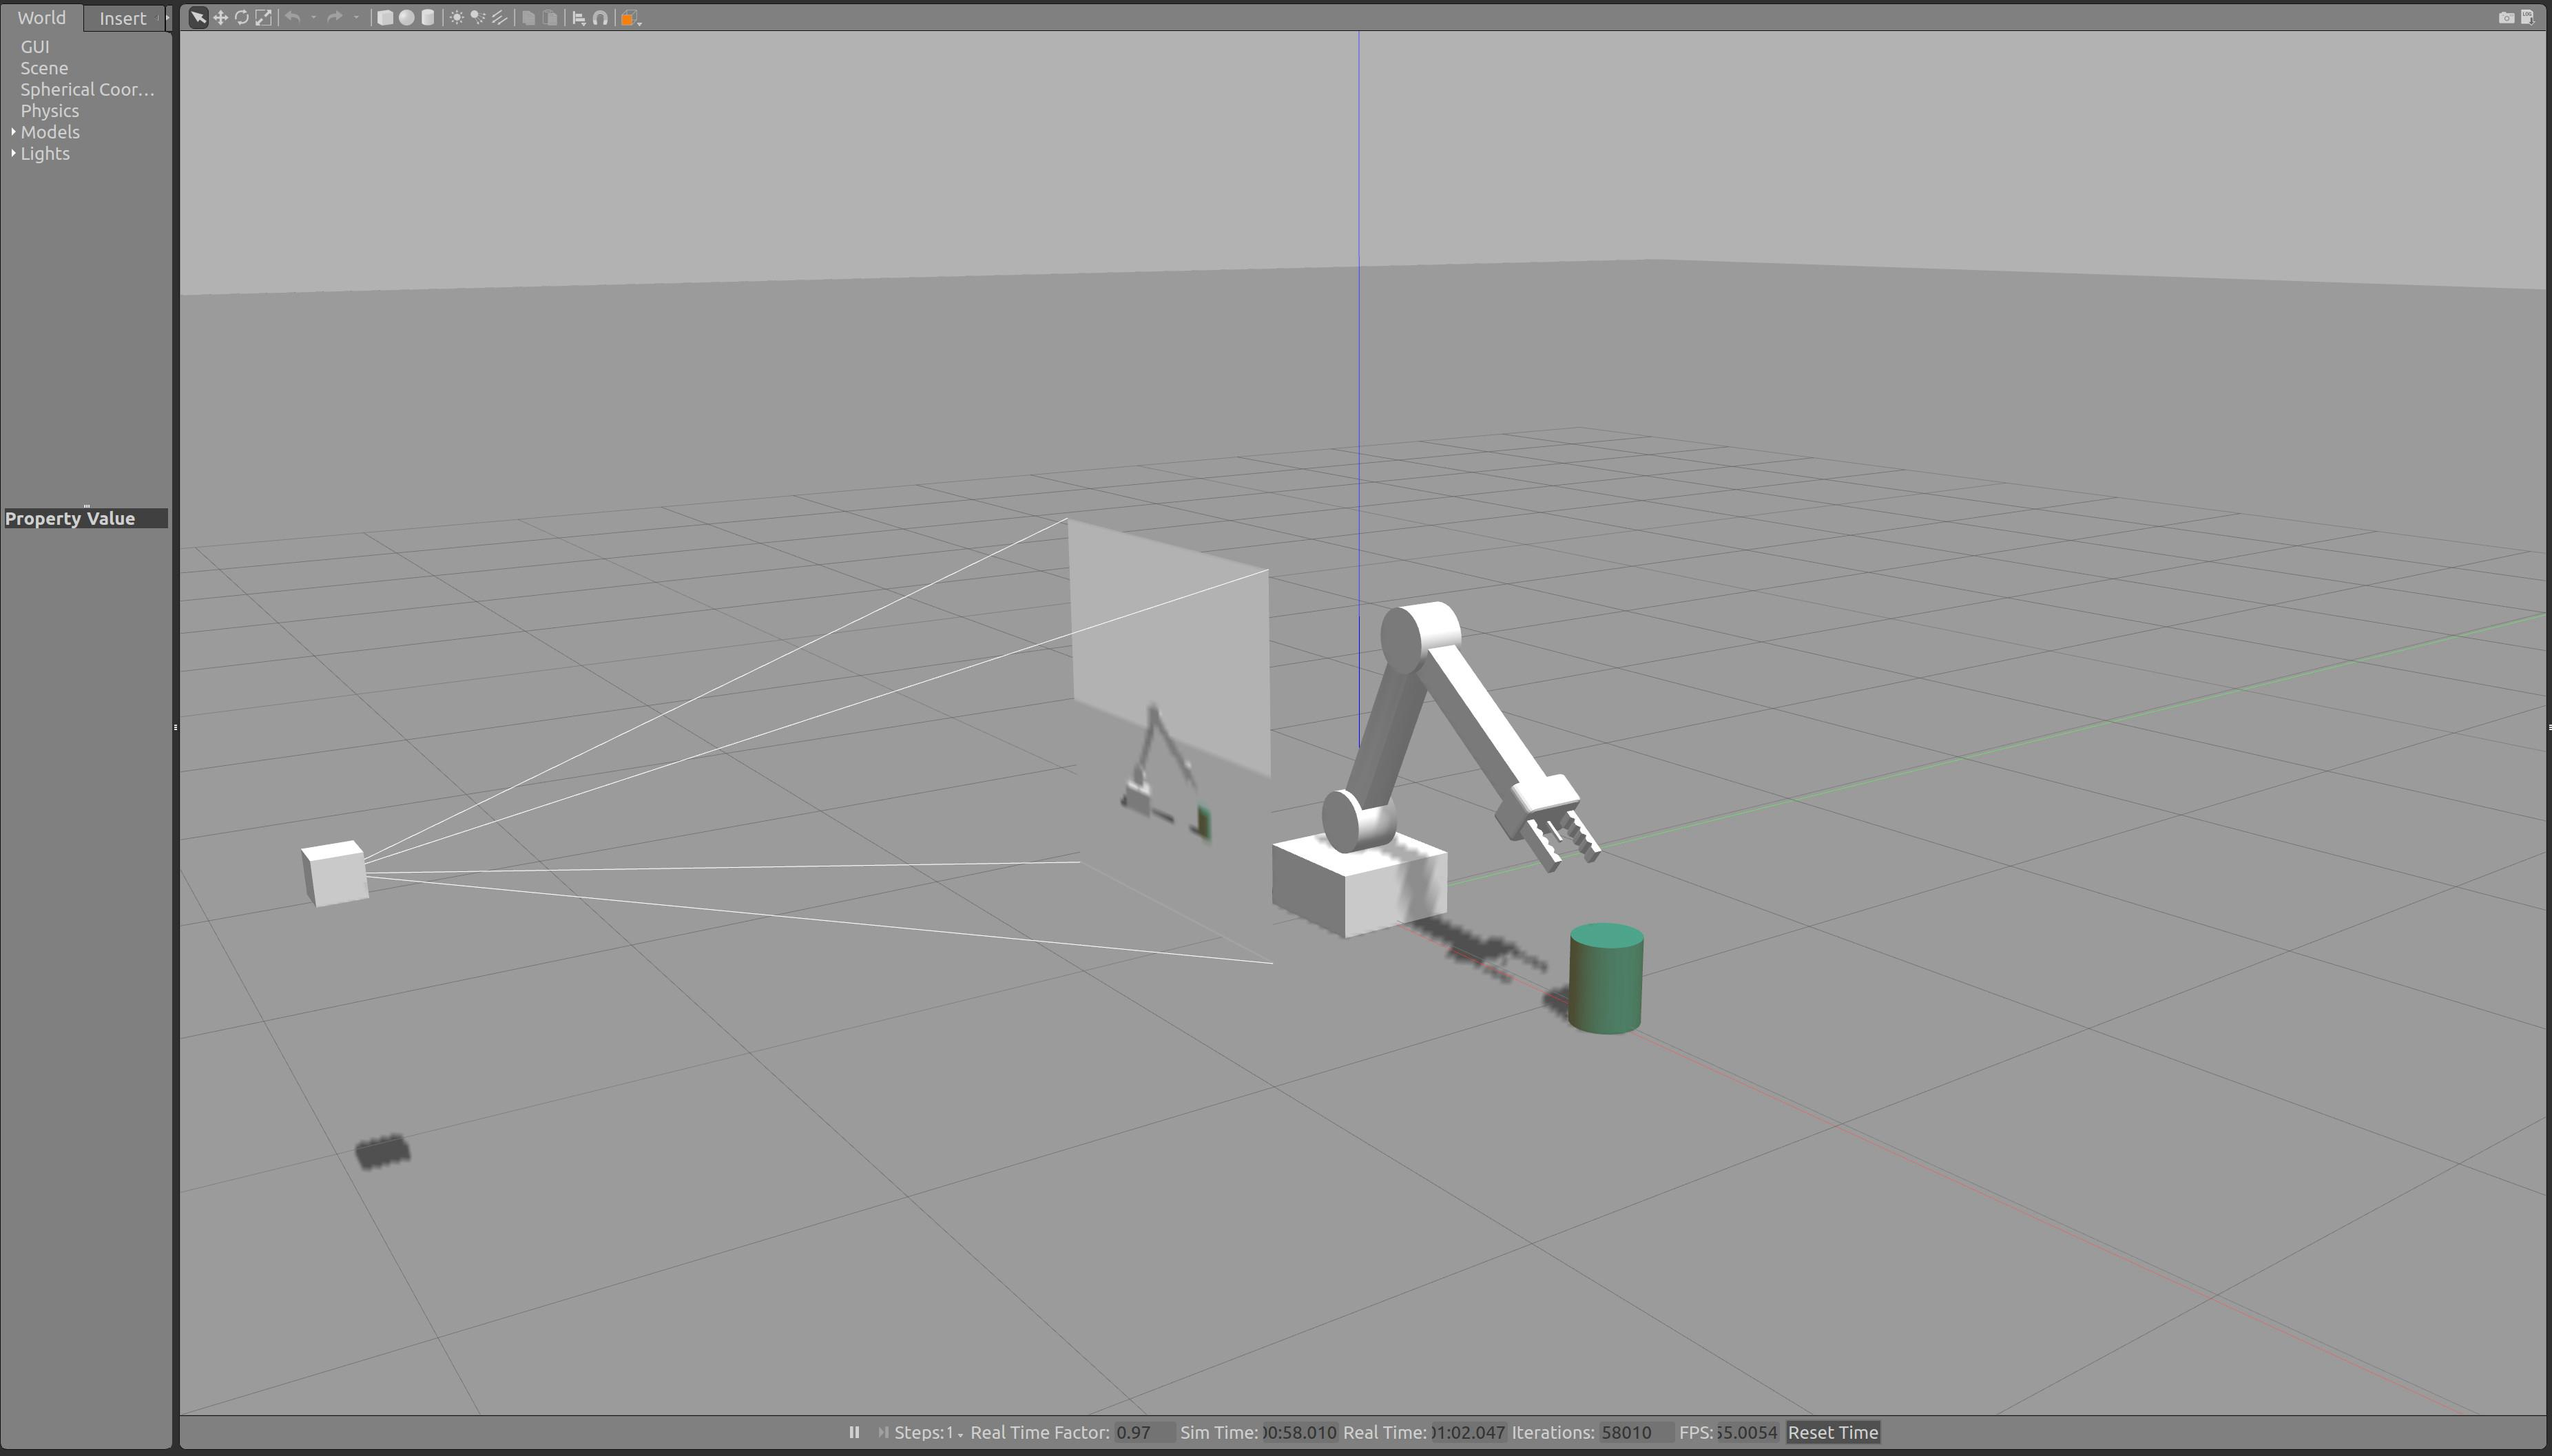
\includegraphics[height=5cm]{imagenes/cap3/2_gazebo_example.JPEG}
	\end{center}
	\caption[Ejemplo de uso de Gazebo]{Ejemplo de uso de Gazebo}
	\label{fig:gazebo}
\end{figure}

\subsection{Rviz}
\label{subsec:rviz}

Por el otro lado, se encuentra \emph{rviz}, que es un visualizador 3D diseñado para la depuración de aplicaciones \ac{ROS} \cite{rviz-def}.\\

En nuestro caso, nos permitirá ver como se dispersa la señal \ac{RF}, que trayectoria y orientación sigue el dron, que efecto tiene sobre la señal la presencia de obstáculos, y otras tantas opciones.\\

\begin{figure} [H]
	\begin{center}
	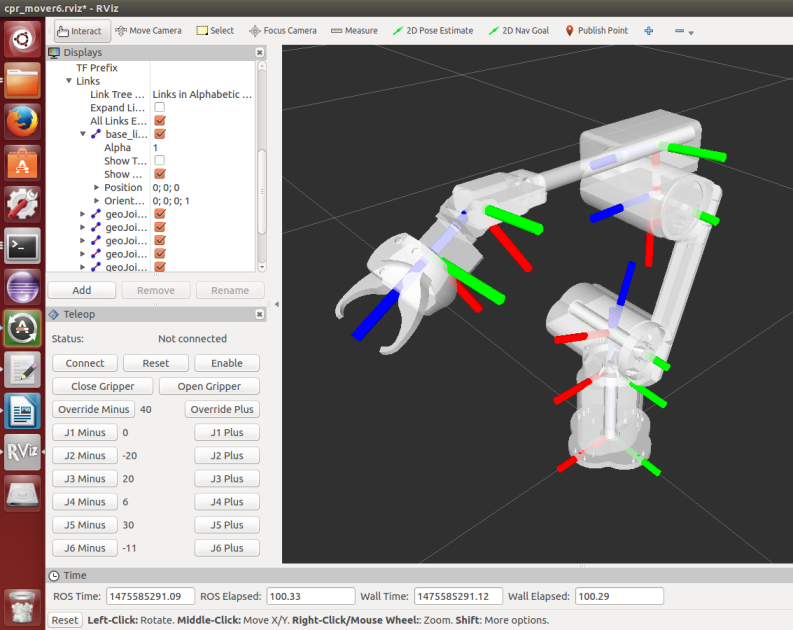
\includegraphics[height=5cm]{imagenes/cap3/3_rviz_example.png}
	\end{center}
	\caption[Ejemplo de uso de Rviz]{Ejemplo de uso de Rviz}
	\label{fig:rviz}
\end{figure}

\section{Plataformas de programación}
\label{sec:plataformas_de_programacion}

\subsection{Visual Studio Code}
\label{subsec:visual_studio_code}

Entre las plataformas usadas para programar, \emph{Visual Studio Code}, o mejor conocido como \emph{VS code}, es un editor de código ligero, funcional tanto en Linux, Windows y macOS \cite{vscode-def}.\\

Su principal ventaja, es que es altamente personalizable a el tipo de desarrollo software que se desee realizar. Todo ello a través de las múltiples extensiones que ofrece, así como la conexión directa y fluida con plataformas como Github, que se detallarán a continuación.\\

\begin{figure} [H]
	\begin{center}
	
\includegraphics[height=3cm]{imagenes/cap3/4_vscode_logo.png}
	\end{center}
	\caption[VS Code logo]{VS Code logo}
	\label{fig:vscode}
\end{figure}

\subsection{Github}
\label{subsec:github}

Github nace de la herramienta \textbf{git}, creada por Linus Torvalds (desarrollador de Linux), que es un sistema de control de versiones, que funciona a grandes rasgos a través de repositorios (o lugares donde se almacenan los sistemas de versiones de forma local), y commits (que permiten actualizar la version del código almacenado del repositorio) \cite{github-def}.\\

Sabiendo esto entonces, ¿qué es github?. Consiste en trasladar la idea de, en vez de tener repositorios locales, que estén distribuidos en una plataforma online, donde además se permita el desarrollo conjunto de aplicaciones de manera distribuida.\\

Por ello, el papel que toma en este proyecto es de vital importancia, ya que asegura un seguimiento y una seguridad, de cara a tener copias de seguridad, donde todo el que desee puede acceder a ver en que punto se encuentra el \ac{TFG} pueda hacerlo.\\

\section{Módulos}
\label{sec:modulos}

\subsection{OpenCV}
\label{subsec:opencv}

Es una biblioteca software de python, enfocada a visión artificial, que dispone de métodos para desarrollar interfaces gráficas de manera intuitiva \cite{opencv-def}.\\

Inicialmente se usó para esto último, por su sencillez y porque se implementó una cámara al dron, de cara a una posible extensión de su funcionalidad en algún punto del proyecto.\\

\begin{figure} [H]
	\begin{center}
	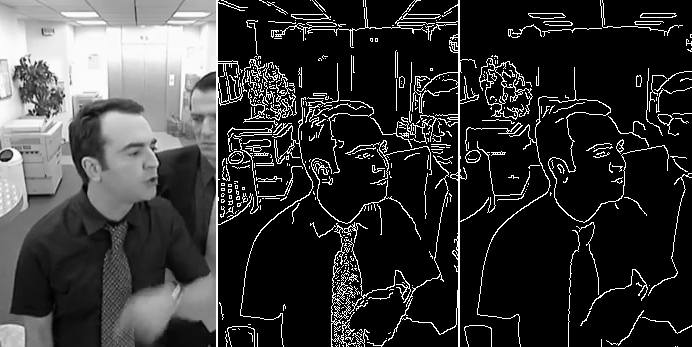
\includegraphics[height=2.5cm]{imagenes/cap3/5_opencv_example.png}
	\end{center}
	\caption[Ejemplo de uso OpenCV (detección de bordes)]{Ejemplo de uso OpenCV (detección de bordes)}
	\label{fig:opencv}
\end{figure}

\subsection{Matplotlib}
\label{subsec:matplotlib}

Presentada por John Hunter en 2002, se usó como biblioteca python alternativa a la anterior mencionada. La gran diferencia radica en que está diseñada para trabajar con estructuras numéricas del tipo array (muy compatible con Numpy \footnote{\url{https://numpy.org/about/}}), lo que permite ofrecer una gran visualización y una interfaz responsiva \cite{matplotlib-def}.\\

En el caso concreto del proyecto, se usó para desarrollar interfaz gráfica, que simula y muestra el comportamiento de una señal \ac{RF}, permitiendo modificar los parámetros de la ecuación en tiempo real.\\

\begin{figure} [H]
	\begin{center}
	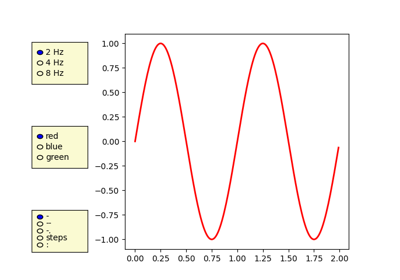
\includegraphics[height=3.5cm]{imagenes/cap3/6_matplotlib_app.png}
	\end{center}
	\caption[Aplicación hecha en Matplotlib]{Aplicación hecha en Matplotlib}
	\label{fig:matplotlib}
\end{figure}

\subsection{PX4 autopilot}
\label{subsec:px4}

Es la capa de software que permite hacer funcionar las aeronaves con sus componentes, esto es a través del controlador de vuelo, que a efectos prácticos se trata del cerebro del sistema, es decir, interconecta los sensores y actuadores, permitiendo comandar diversas acciones \cite{flight-controller} \cite{px4-def}.\\

Este sistema, usa un conocido protocolo de comunicaciones llamado \textbf{MAVLink}, que se encarga de gestionar la comunicación entre el controlador de vuelo y la \ac{GCS}. En nuestro caso, y como queremos desarrollar aplicaciones mediante \ac{ROS}, debemos añadir una capa más, que se encarga de traducir los mensajes ROS a mensajes compatibles con el protocolo MAVLink, y de esto se encarga \textbf{MAVROS} \cite{px4-mavlink} \cite{px4-mavros}.\\

\begin{figure} [H]
	\begin{center}
	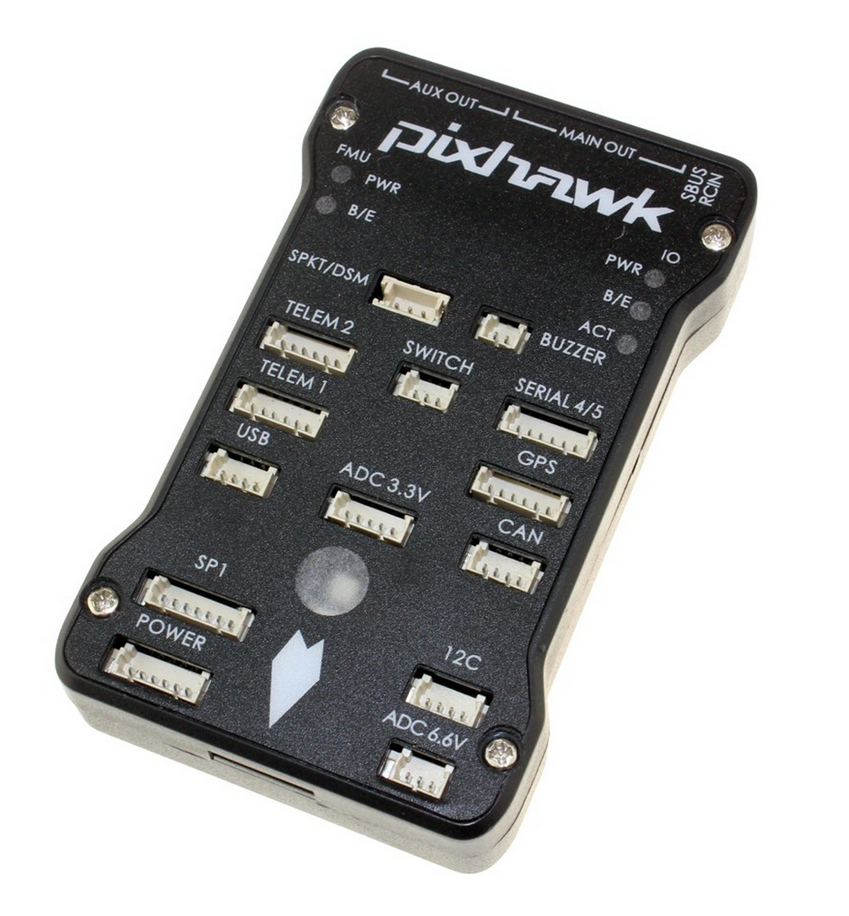
\includegraphics[height=2.5cm]{imagenes/cap3/7_px4_logo.png}
	\end{center}
	\caption[PX4 Autopilot logo]{PX4 Autopilot logo}
	\label{fig:px4autopilot}
\end{figure}

\section{Iris}
\label{sec:iris}

Es el nombre de la aeronave usada para solucionar los problemas planteados. En síntesis, es un dron cuadracóptero provisto de una cámara y un sensor de \ac{RF} simulado. Dicha aeronave es cortesía de \textbf{JdeRobot}, que es un conjunto de herramientas pensadas para desarrollar aplicaciones robóticas \cite{jderobot-ref}.\\

\begin{figure} [H]
	\begin{center}
	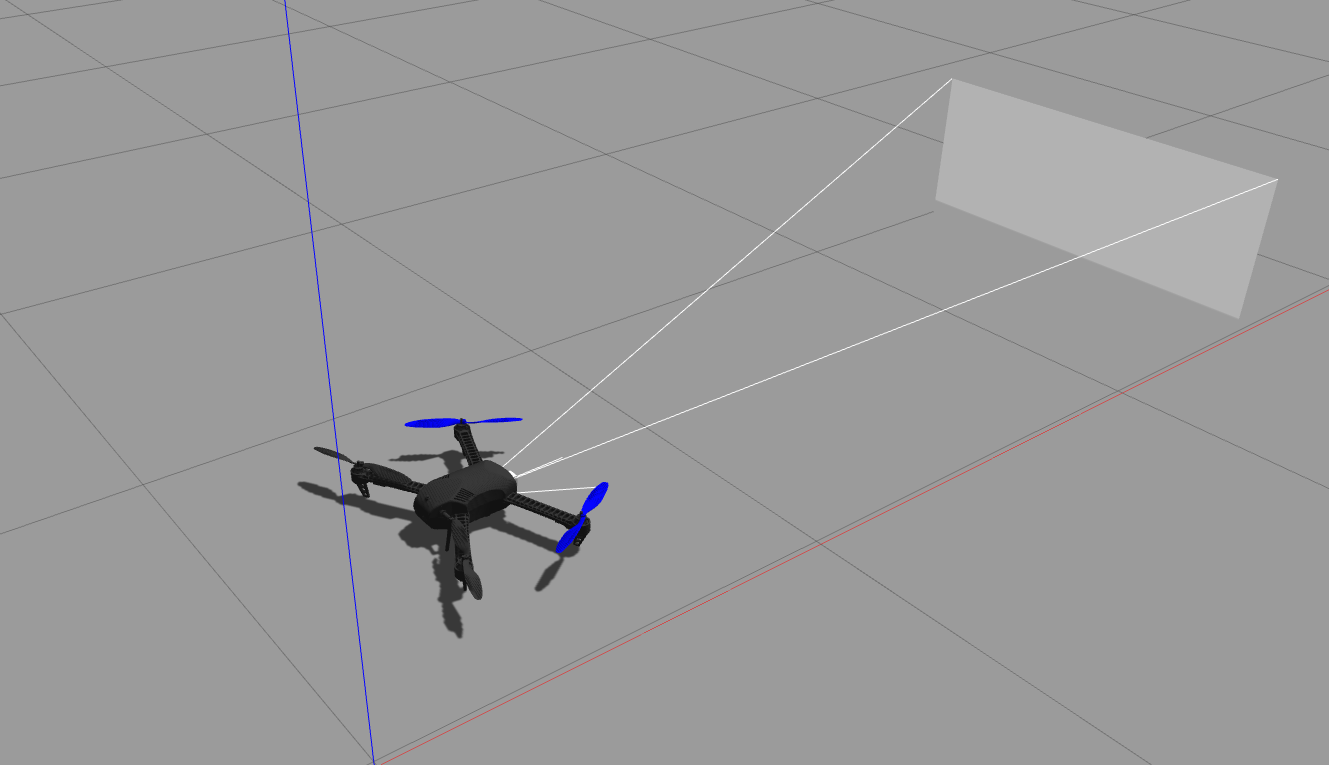
\includegraphics[height=5cm]{imagenes/cap3/8_iris_drone.png}
	\end{center}
	\caption[Iris drone en Gazebo 11]{Iris drone en Gazebo 11}
	\label{fig:irisdrone}
\end{figure}